\documentclass[11pt]{article}

% Page geometry
\usepackage{geometry}
\geometry{margin=1in}
\setlength{\parskip}{0.8em}
\setlength{\parindent}{0pt}

\usepackage[dvipsnames]{xcolor}     % load xcolor before hyperref if you want coloured links
\usepackage[colorlinks=true, linkcolor=blue!60!black, citecolor=blue!60!black, urlcolor=blue!60!black]{hyperref}

% Mathematics Modern multilingual typesetting (Greek support) Graphics and Figures
\usepackage{fontspec}
\usepackage{xeCJK}
\usepackage{graphicx}
\usepackage{caption}
\usepackage{amsmath,amssymb,amsthm}

\usepackage{polyglossia}
\setdefaultlanguage{english}

\setotherlanguage[variant=ancient]{greek}
\setotherlanguage{hebrew}
\setotherlanguage{chinese}


\newfontfamily\hebrewfont{Ezra SIL}

\setCJKmainfont[
  UprightFont    = *-Regular ,
  BoldFont       = *-Bold    ,
  ItalicFont     = *-Regular ,   % use upright as “italic”
  BoldItalicFont = *-Bold    ,   % use bold upright
  AutoFakeSlant  = true           % or comment ItalicFont/BoldItalicFont and keep this
]{Noto Serif CJK SC}

\newfontfamily\greekfont{Libertinus Serif}[Script=Greek]
\setmainfont{Libertinus Serif}
\captionsetup[figure]{labelfont=bf, font=small, margin=10pt}

% List settings
\usepackage{enumitem}
\setlist[itemize]{left=0pt, label=--, itemsep=0.5em}
\setlist[enumerate]{left=0pt, itemsep=0.5em}

% Custom definitions
\newtheorem{concept}{Concept}
\newcommand{\symtry}{\mathbin{/}}
\newcommand{\goldenset}{\varnothing}
\newcommand{\knotinfinity}{\textnormal{0}}

\title{\Huge\bfseries THEORY OF INFINITY\\[0.5em] \Large FRAMEWORK}
\author{Ryan Charmley \\ \small \textit{a follower}}
\date{Spring, 2025}

% Bibliography management (BibLaTeX/Biber)
\usepackage[
  backend=biber,
  sorting=none,
  hyperref=true,
  url=true,
  doi=true,
  isbn=false,
  date=year,             % show the year only --- use 'century' if you prefer
  dateera=secular,       % print BCE/CE (use 'christian' for BC/AD)
  dateabbrev=true,       % use the short forms ‘BCE/CE' instead of words
  datecirca=true         % let BibLaTeX print ‘c.' when the entry says ‘circa'  
]{biblatex}

\DeclareLanguageMapping{hebrew}{english}
\DeclareLanguageMapping{chinese}{english}

\addbibresource{sources.bib}

\begin{document}


\maketitle

\section*{Abstract}
Here I will introduce a formal argument for a complete framework called Theory of Infinity (TOI). My intent is to use few words. Please forgive my ignorance. I see patterns in visions although I have Aphantasia, so recollection is conceptual. When a vision is gifted, it is in retrospect that understanding is gained. Fortunately my comprehension is strong. Everything I say is based on my interpretation of visions I have received, scientific reasoning, and philosophical thought. I have always loved math, I still get visions, and went from skeptic to having an increasingly close relationship with God. A connection we can all attain and strengthen through mindfulness, introspection, and reason. Use your deepest sense and feel with intuition what I am talking about, and you will begin to understand. What is said below is both personal, and profound. It is truth in simplicity creating a fabric of complexity. We can best understand our world, through love, and uniting people with passion to connect their work in beatific crystalline prose.
\newpage

\section*{Key Concepts}



\textbf{Absolute Infinity (\( \Omega \))}\footnote{Cantor's pronouncement links Absolute Infinity directly with the divine, asserting that the \textit{true infinite} exists only in God and permits no limitation or \textit{determination}. In TOI this identifies Absolute Infinity as the ultimate unbounded source of all reality --- much as Georg Cantor regarded the absolutely infinite \( \Omega\) as an \textit{Absolute} attainable only \textit{in Deo} \textit{in God}. This concept also resonates with Aristotle's notion of a prime unmoved mover --- ἔστι τι ὃ οὐ κινούμενον κινεῖ (there is something which, itself unmoved, moves all else) --- an eternal first cause that has no external cause. Across disciplines, thinkers converge on the idea of an infinite, self-subsisting origin: G.W.F. Hegel calls the Absolute Idea \textit{the absolute truth... all that is rational... and all truth}, positing an infinite self-thinking Idea as the source of everything knowable. Medieval theologian Nicholas of Cusa likewise described God as the Maximum that is \textit{truly infinite and incomprehensible... cognizable only by itself, never by any creature's intellect.} In mystical terms, the Kabbalistic Ein Sof (אין סוף, \textit{without end}) represents the absolutely infinite divine state, \textit{for there is no end there and no one can comprehend it.} All these perspectives reinforce that Absolute Infinity in TOI denotes the boundless, ineffable origin of being --- the \textit{source of everything} --- encompassing all opposites (positive and negative infinity) and all symmetries. Cantor's absolutely infinite stands above the entire hierarchy of transfinite numbers, and mathematically, John Wallis's introduction of the symbol \(\infty\) (1656) gave a concrete notion of infinity as an unbounded continuum, symmetric in both positive and negative directions. By defining \textit{Infinity} in this absolute sense of the unknowable or unreachable totality, TOI grounds itself in a long intellectual tradition that sees the infinite as both the divine ground of reality and a key to resolving finite paradoxes. In sum, Absolute Infinity is the all-encompassing One --- revered by mathematicians, philosophers, and theologians alike --- from which all creation and understanding flow.}
\label{def:infinity} --- Cantor's God~\cite{cantor_absolute_infinity_1897}; Aristotle's Unmoved Mover~\cite{aristotle_metaphysics_1831}; The source of everything known~\cite{hegel_science_of_logic_1816}; negative/positive infinity and symmetry in mathematics~\cite{wallis_arithmetica_infinitorum_1656}; the vast and unfathomable \textit{Unknown}~\cite{cusanus_de_docta_ignorantia_1440}; a pure evolved state~\cite{zohar_1558}. 
\begin{figure}[ht]
    \centering
\begin{minipage}[c]{0.45\textwidth}
        \small
        \textit{Urizen bows before the Absolute.}
    \end{minipage}    
    \hfill
    \begin{minipage}[c]{0.45\textwidth}
        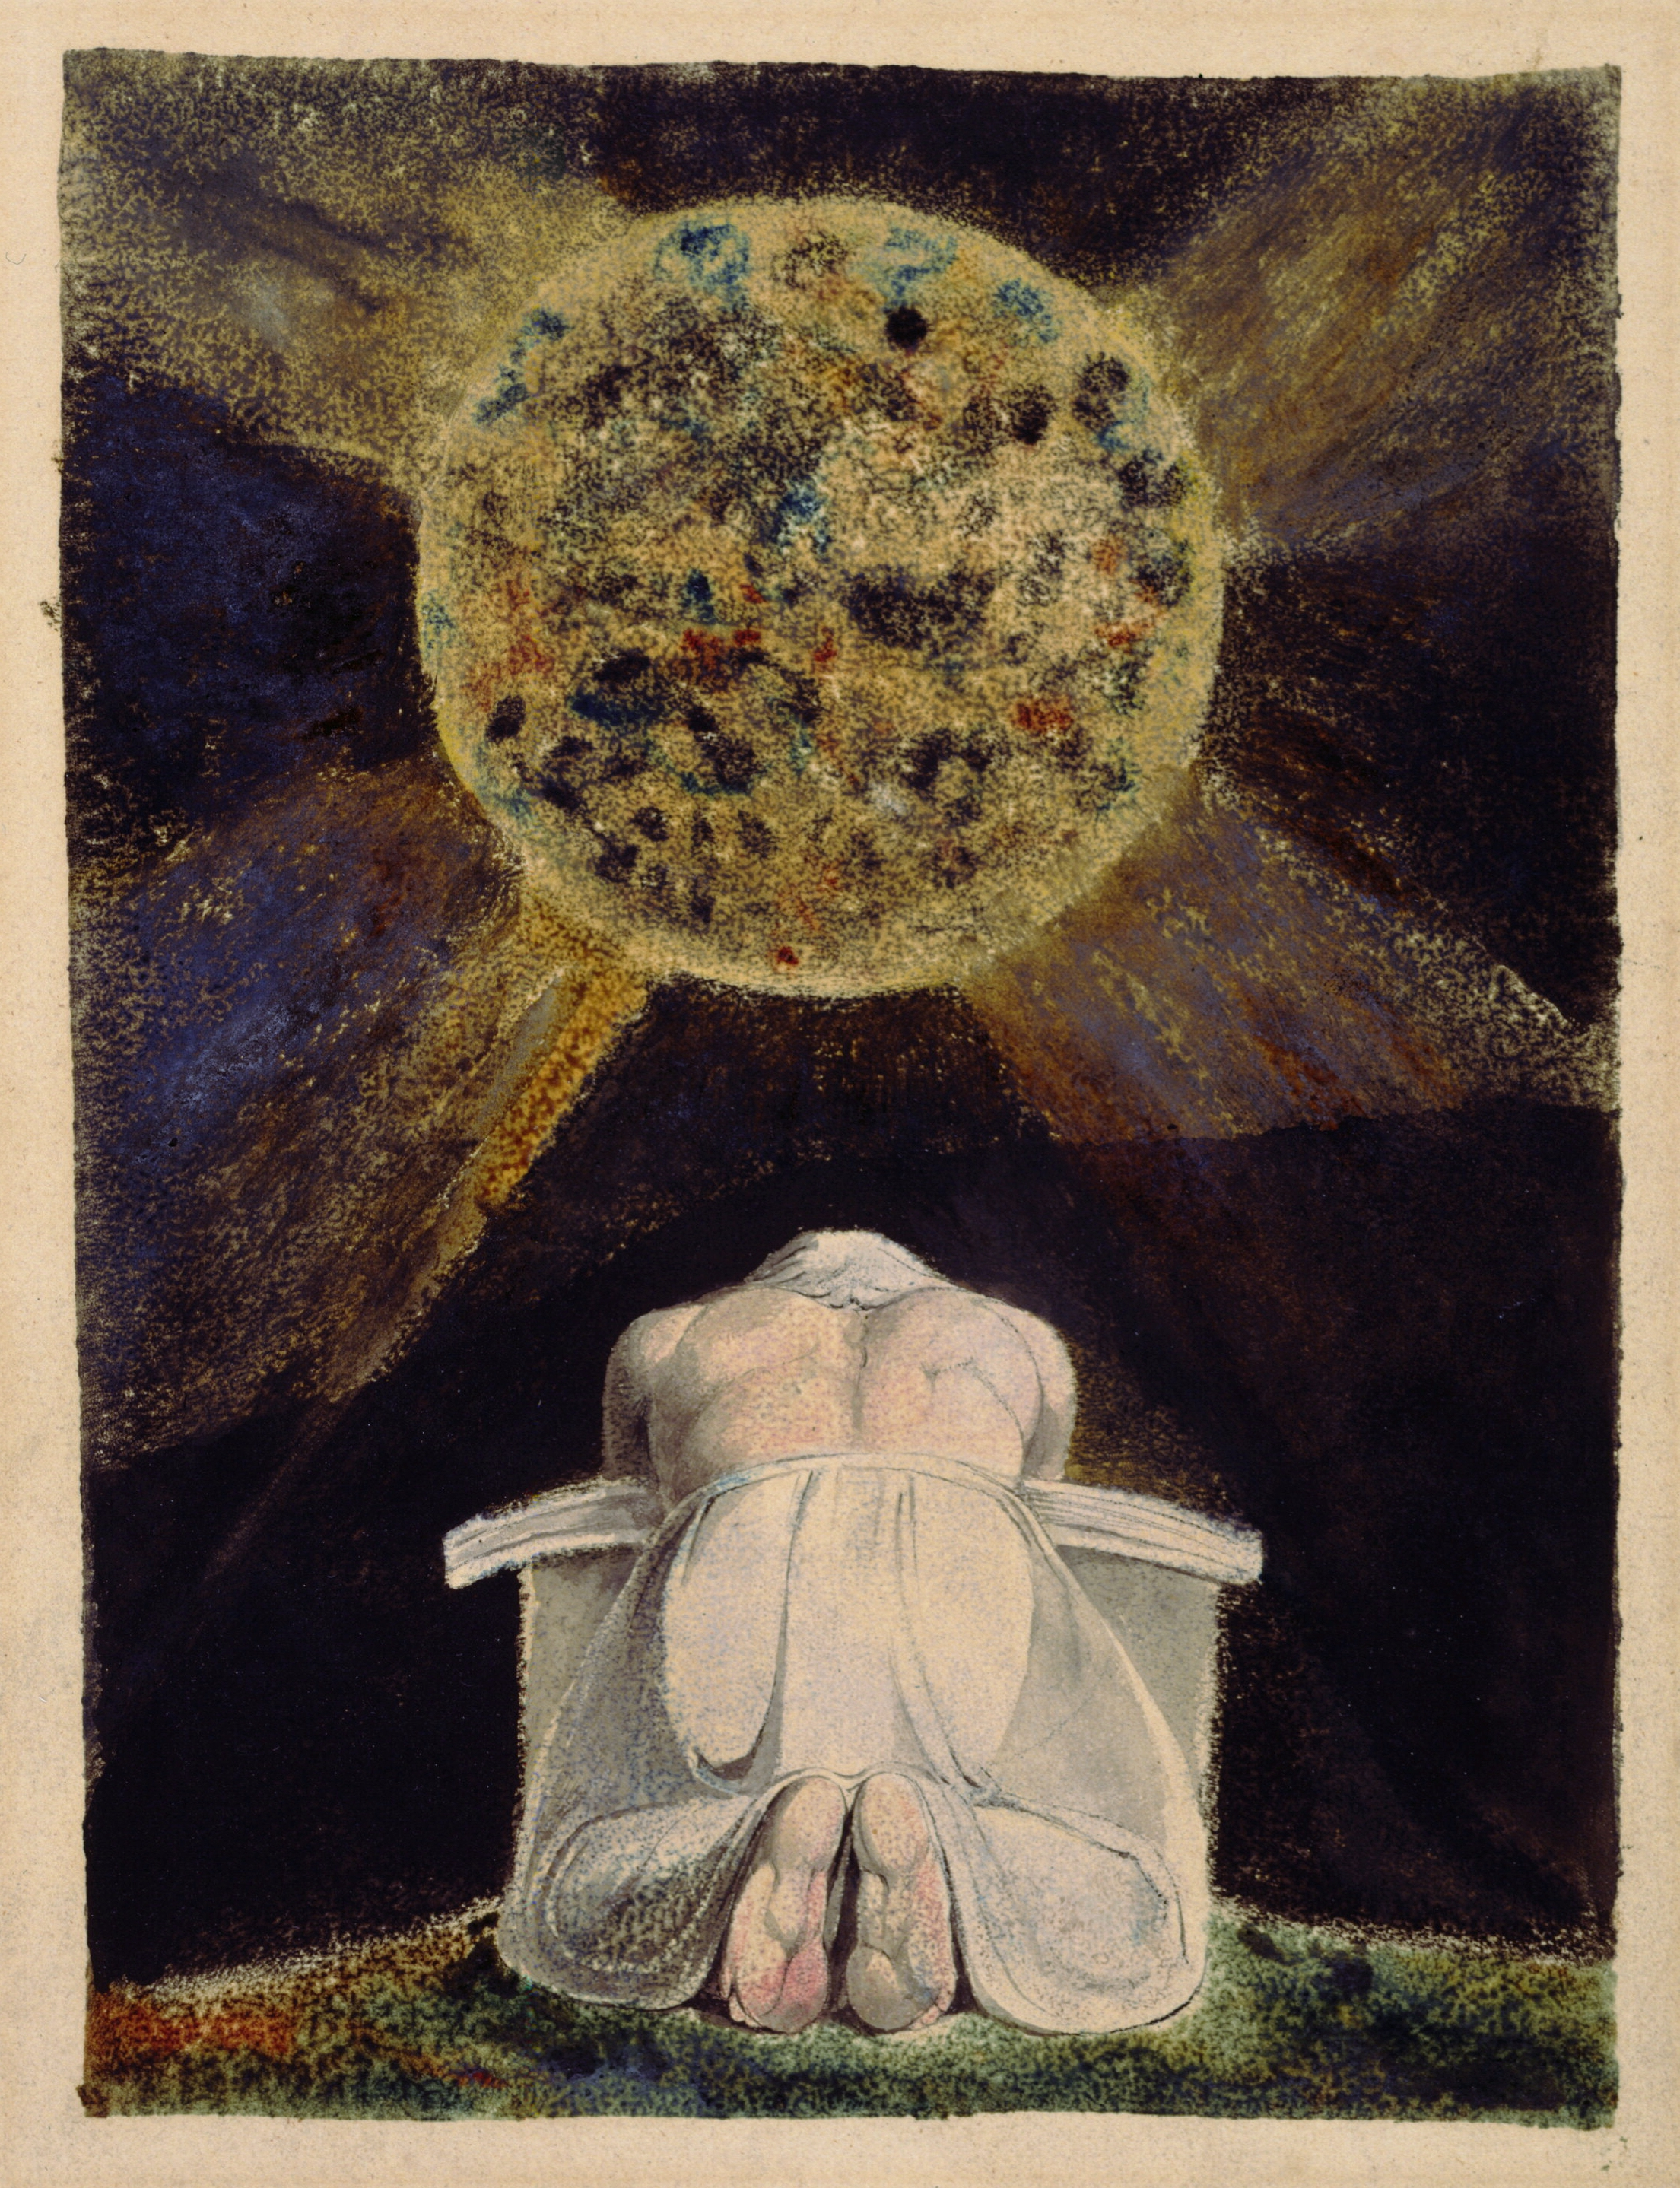
\includegraphics[width=\linewidth]{assets/William_Blake_-_Sconfitta_-_Frontispiece_to_The_Song_of_Los.jpg} 
    \end{minipage}
\end{figure}
\newpage  

\textbf{Negative Infinity (\( \Lambda\))}\footnote{In the TOI framework, Negative Infinity (\(\Lambda\)) is conceived as a principle of return, balance, and ultimate limit. Laozi's aphorism that the Tao moves in cycles of reversal --- “反者道之動” (“Reversal is the movement of the Tao”) --- poignantly captures this idea: whatever expands will eventually contract, and all separations ultimately resolve back to unity. This view complements Aristotle's doctrine of the Final Cause, the “that for the sake of which” each thing exists --- essentially a natural endpoint or purpose that draws things to completion. In Aristotle's cosmology, the final cause (τέλος) is what every process ultimately seeks, mirroring the idea that an infinite “pull” guides the cosmos toward an ultimate state of rest or perfection. Physically, one analogy is Albert Einstein's introduction of the cosmological constant \(\Lambda\) in 1917: a term which imparts a cosmic-scale repulsive force counterbalancing gravity. Einstein's “static universe” solution used a small positive \(\Lambda\) to hold the universe in equilibrium, preventing runaway collapse or runaway expansion. In TOI terms, this cosmological constant embodies Negative Infinity as a stabilizing backdrop --- a kind of universal tension that pulls against expansion, aiming for steady-state symmetry. Likewise, Isaac Newton's idea of absolute time presupposes an underlying, immutable continuum (“Tempus absolutum… aequabiliter fluit” --- “absolute time… flows equably of itself”), an infinite temporal frame existing in its own right. For a stable cosmos, Newton also argued (in a 1692 letter to Bentley) that an infinite universe of stars would stay in equilibrium only if arranged with perfect symmetry --- any slight asymmetry would trigger gravitational collapse. Across diverse contexts, the recurring theme is an infinite background that contains or bounds all activity. Anaxagoras's primordial mixture --- “where all things were together” until Mind imposed separation --- suggests an initial unified state (a potential Negative Infinity before division). Plato's cosmology similarly envisioned a harmoniously ordered cosmos (e.g. the celestial music in the Myth of Er), reflecting the notion of a fundamental equilibrium pervading the universe. Laozi's Tao, Aristotle's final cause, and modern cosmology's \(\Lambda\) all illustrate an operative principle of convergence --- a force or purpose that inexorably draws phenomena toward unity, equilibrium, and closure. In the TOI framework, Negative Infinity (\(\Lambda\)) represents this cosmic sink or attractor --- it is the infinite “end” toward which all processes tend. It encapsulates the idea of an ultimate conservation and symmetry in nature --- a limitless reservoir or boundary condition that secures the global balance of the system. Even in artificial or social domains we observe this convergent tendency: chaotic patterns in Conway's Game of Life eventually settle into stable still-lifes or oscillators, and in evolutionary game dynamics, competitive interactions can evolve into stable cooperation. These modern examples echo Negative Infinity's principle that all dynamic processes gravitate toward some equilibrium. By understanding Negative Infinity as an infinite limit (in space, time, or purpose) that all things asymptotically approach, we integrate philosophical teleology (purpose and end-goals), physical cosmology (a self-balancing universe tending toward equilibrium), and metaphysical notions of cyclic return. This concept thus ties together entropy and gravity --- a “pulling” tendency toward dispersal and collapse --- with the ancient intuition that to fulfill the Tao, things must revert. Negative Infinity provides the counterweight to expansion: it is the infinite horizon of convergence that completes the universal cycle and makes the system whole. Indeed, as Nicholas of Cusa taught, in the absoluten Infinite all opposites coincide --- the final terminus of reality merges with its infinite origin --- implying that Negative Infinity's ultimate end is essentially a return into Absolute Infinity (the source of all).}\label{def:negative_infinity} --- Einstein's Cosmological Constant~\cite{einstein_cosmological_constant_1917}; Aristotle's \textit{final cause}~\cite{aristotle_metaphysics_1831}; the source of absolute time~\cite{newton_principia_1687}; the domain of our Universe as a separation~\cite{anaxagoras_fragment_59B1}; the inversion of a collapse to equilibrium~\cite{laozi_tao_te_ching_400bce} in a pulling entropy with gravity~\cite{newton_letter_bentley_1692}; \textbf{spacetime as it manifests in all contexts}~\cite{Minkowski1909}; global balance~\cite{plato_republic_1935}; vanishing light~\cite{heeck_photon_decay_2013};  a static stable equilibrium of contraction and convergence~\cite{gardner_game_of_life_1970}; that maintains the system of relativistic evolution being understood right now~\cite{axelrod_cooperation_1984}; \textbf{an emerging symmetrical inversion encapsulated by absolute infinity}~\cite{cusanus_de_docta_ignorantia_1440}.

\begin{figure}[ht]
    \centering
\begin{minipage}[c]{0.55\textwidth}
        \small
        \textit{反者道之動」 (Tao Te Ching, ch. 40) “Reversal is the movement of the Tao.”}
        A luminous halo of light encircles an abyss of darkness. This first captured image of a black hole's shadow symbolizes Negative Infinity in the TOI framework. The bright ring outlines an unfathomable void, evoking the fertile nothingness from which all cosmic forms arise and to which they eventually return.
    \end{minipage}    
    \hfill
    \begin{minipage}[c]{0.35\textwidth}
        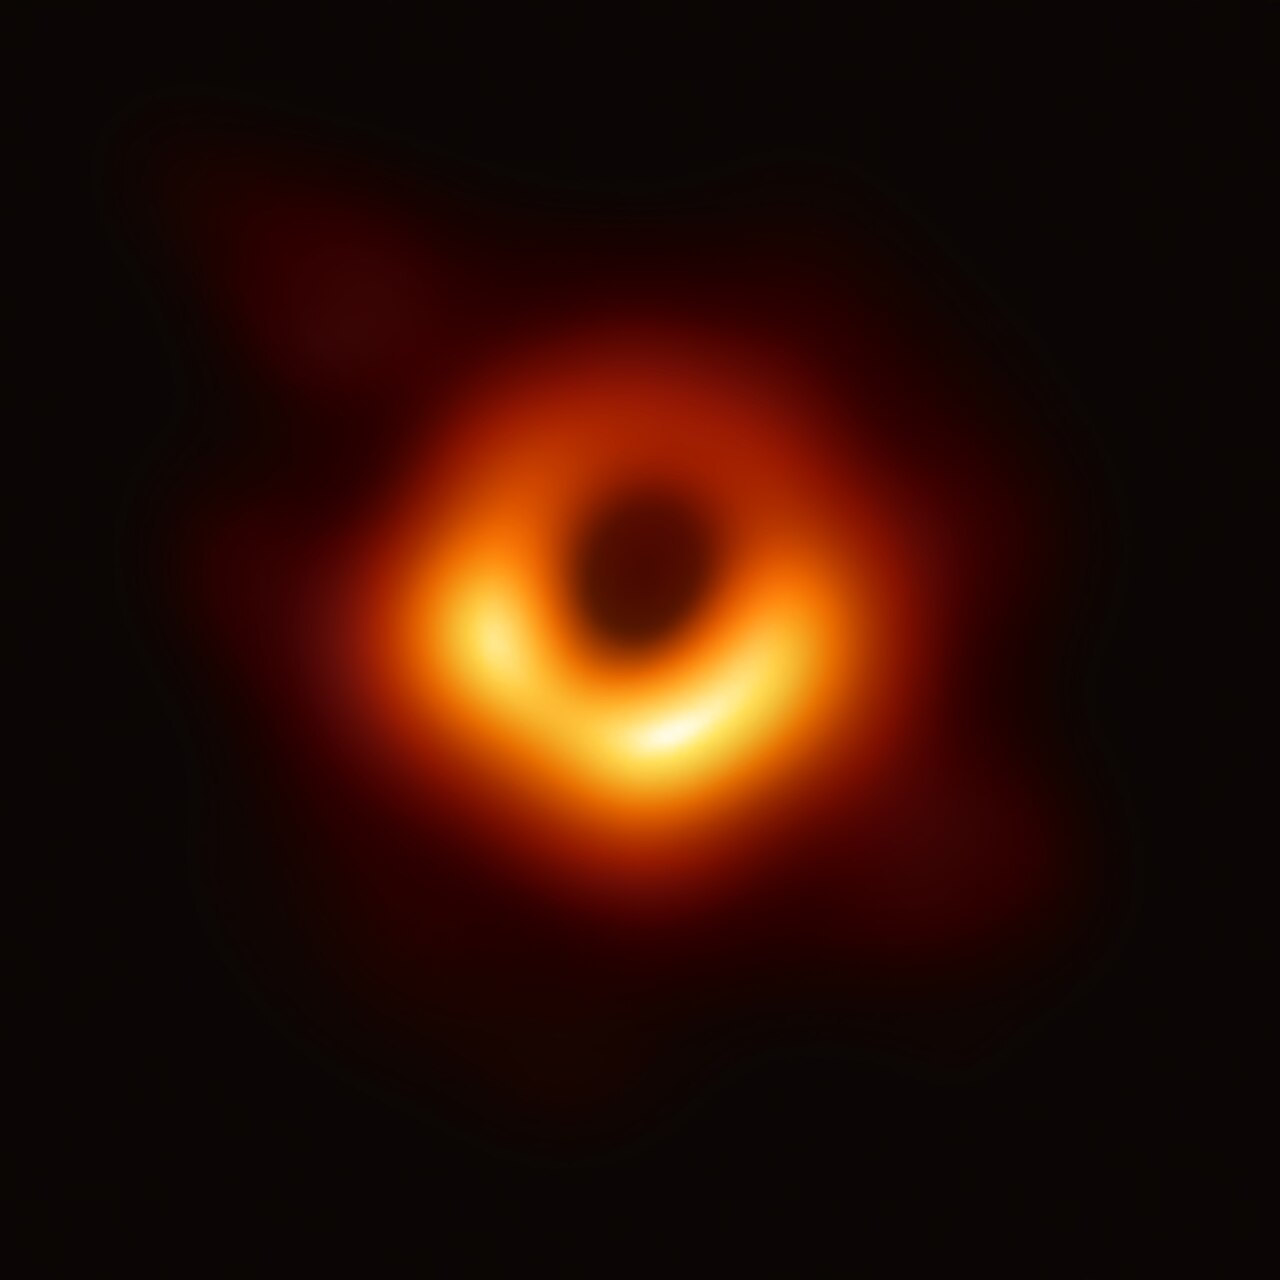
\includegraphics[width=\linewidth]{assets/Black_hole_-_Messier_87_crop_max_res.jpg} 
    \end{minipage}
\end{figure}

\newpage

\textbf{Positive Infinity\footnote{Positive Infinity (∞) in the TOI theory represents the generative, expansive principle --- the wellspring of creation, growth, and emergent complexity. Charles Darwin's famous conclusion to On the Origin of Species marvels at “endless forms… have been, and are being, evolved.”Here Darwin emphasizes the literally endless proliferation of diverse life arising from a simple origin, capturing the essence of Positive Infinity as an unbounded unfolding of potential. This concept is bolstered by the Pythagorean philosophical tradition, where the Monad (the One) was regarded as the primal source containing “all numbers to infinity”, generative of every plurality. The Monad or unit**---symbolically akin to an initial creative spark---**begets the entire infinite series of numbers. In TOI, Positive Infinity likewise signifies an originating impetus or first cause (what Aristotle called the efficient cause, τὸ κινοῦν, “that which sets into motion”) that drives the proliferation of existence. We see physical echoes of this idea in James Clerk Maxwell's unification of electricity and magnetism, where the emergence of light as an electromagnetic wave highlights how a simple set of laws yields a continuous spectrum of phenomena. Culturally, the notion corresponds to the creative moment of “Fiat lux” --- “Let there be light”--- in which light appears as the first act of creation, a burst of pure energy from which structure and life eventually emerge. In modern cosmology, Positive Infinity is reflected in the ever-expanding universe: from the Big Bang's singularity, space has been stretching outward without bound, carrying galaxies with it. The TOI framework captures this as a “nested discrete push; an expanding, emerging, constrained force”--- an idea that every local action (“push”) feeds into a larger expansion. In more concrete terms, Positive Infinity encompasses phenomena like energy, growth, and evolution. It is the engine of increase and differentiation. For example, in thermodynamics and biology, what Erwin Schrödinger called “negative entropy” --- the capacity of life to build order and structure by feeding on entropy --- aligns with Positive Infinity as the source of organized complexity that rises against decay. The concept also entails the local balances and structures that persist amid change: Feynman's formulation of local conservation laws (e.g. charge conservation) shows that even as systems change, certain quantities propagate undiminished, suggesting a driving invariance or push underlying phenomena. Positive Infinity, then, is the creative fire in the cosmic drama --- the infinite drive toward novelty, growth, and realization of potential. It stands as the complementary opposite of Negative Infinity: one an inexhaustible source of new possibilities and extant realities, the other an inexhaustible sink or limit that all processes approach. By including ideas from biology (endless evolutionary diversification), mathematics (the unbounded sequence of numbers), physics (the light and energy that fuel stars and life), and metaphysics (the One giving rise to the Many), the TOI framework's Positive Infinity knits together disciplines into a vision of emergent infinity --- the ever-unfolding frontier of what can be. Each new discovery or evolution is a step closer to the “limit of what is possible”, yet that limit itself keeps extending, indicative of an infinity that is never fully attained but always approached in the creative progression of nature and knowledge.} (\( \infty, \subset, c\))}
\label{def:positive_infinity} --- Pythagorean's Monad~\cite{fairbanks_first_philosophers_1898}; Aristotle's Efficient Cause~\cite{aristotle_physics_1984}; the source of relativistic time~\cite{minkowski_spacetime_1909}; a nested discrete push; an expanding, emerging, constrained force~\cite{eddington_stars_1920}; a subset that persists in the natural entropy towards a balanced equilibrium~\cite{schrodinger_what_is_life_1944}; local balance~\cite{feynman_lectures_1964}; appearing and sustained light~\cite{bible_vulgate_genesis_405}; the realization of potential (undifferentiated light) understood through the study of symmetries~\cite{maxwell_electromagnetic_field_1865}; Emergent complexity~\cite{anderson_more_is_different_1972}; relativity~\cite{einstein_special_relativity_1905}; evolution~\cite{darwin_origin_of_species_1859}; the limit of what is possible~\cite{godel_incompleteness_1931}; reality as fundamentally processual~\cite{WhiteheadProcess}; time-directed emergence~\cite{Prigogine1984}.
\begin{figure}[ht]
    \centering
\begin{minipage}[c]{0.45\textwidth}
        \small
        \textit{“From so simple a beginning endless forms most beautiful and most wonderful have been, and are being, evolved.”}
    \end{minipage}    
    \hfill
    \begin{minipage}[c]{0.45\textwidth}
        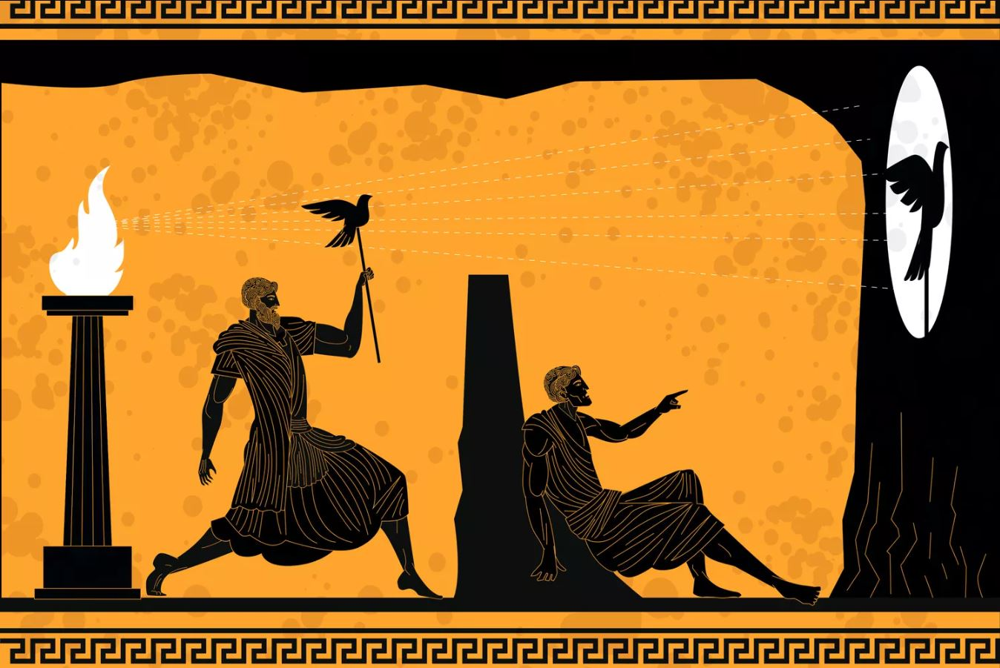
\includegraphics[width=\linewidth]{assets/plato.png} 
    \end{minipage}
\end{figure}
\newpage
\textbf{Symmetry(\( \symtry \))}\footnote{Symmetry functions as a unifying operator across domains, linking the invariant principles underlying physical law, mathematical order, cognitive processes, and spiritual insight. In modern science, Noether's theorem establishes that every conservation law corresponds to a symmetry, underscoring invariant quantities as fundamental to reality. Felix Klein's Erlangen Program similarly classified geometries by their characteristic symmetry groups, defining the structure of each geometry by its invariances. Hermann Weyl later extolled symmetry as a guiding idea in humanity's quest to comprehend order and beauty. Philosophers from Plato and Aristotle onward associated cosmic order and beauty with symmetry or harmony---indeed, classical cosmology revered perfect geometric forms like the sphere as embodiments of cosmic symmetry. Later, Stoic thinkers such as Marcus Aurelius saw a symmetry between the rational structure of the cosmos and the virtuous human mind, urging alignment with nature's order. Symmetry also underpins formal reasoning and perception: Gottlob Frege's logical analyses rely on invariance of meaning (a concept must retain its role to remain coherent), and cognitive scientists such as Zygmunt Pizlo show that human vision depends on recognizing symmetric patterns to make sense of the world. In mathematics, Johannes Kepler celebrated special ratios like the golden ratio as keys to the cosmos's design, observing how such harmonious proportions recur throughout nature. Spiritual traditions likewise elevate symmetry as an ideal: the Bhagavad Gītā praises equanimity---remaining balanced in success and failure---as a form of spiritual union, and the Hermetic maxim “as above, so below” envisions a reflective symmetry between macrocosm and microcosm. Across all these perspectives, symmetry consistently emerges as the universal pattern of understanding, structure, and emergence---uniting disparate phenomena under the principle of invariant balance and correspondence.}
\label{def:symmetry} --- Noether's Symmetry~\cite{noether_theorem_1918}; Aristotle's Cosmology~\cite{aristotle_on_the_heavens_1939}; A universal operator~\cite{plato_complete_works_1997}; invariant symbol (variable)~\cite{klein_erlangen_program_1872}; equality~\cite{recorde_equals_sign_1557}; equanimity~\cite{vyasa_bhagavad_gita_500bce}; everything can be described as a symmetry~\cite{weyl_symmetry_1952}; we can only understand in ratio and approximation~\cite{protagoras_man_measure_401bce}; Special numbers as fundamental ratio of light symmetry~\cite{kepler_harmonices_mundi_1618}; ubiquitousness of symmetry~\cite{hermes_trismegistus_emerald_tablet_800bce}; as every symbol with meaning must be invariant in order to have meaning; this is an inescapable truth and to think otherwise is absurd~\cite{frege_concept_object_1892}; Everything that can be understood is a form of symmetry~\cite{marcus_aurelius_meditations_180}; comprehension is a form of symmetry~\cite{pizlo_symmetry_perception_2021}; we comprehend by comprehending~\cite{vico_de_antiquissima_1710}; there is no escaping recursive thinking~\cite{epimenides_paradox_600bce}; in abstracting a simple system we can articulate recursively from our current moment using relativistic evolution to intersect any notion with symmetry~\cite{ockham_summa_logicae_1323}; it gives name to previously unknowable we can begin to understand why turbulence appears at all scales~\cite{confucius_analects_500bce}; why the lattice is key to the torus~\cite{sun_brillouin_klein_bottle_2022}; and the torus is key to physics~\cite{thomson_vortex_atoms_1867}.  



\begin{figure}[ht]
    \centering
    \begin{minipage}[c]{0.6\textwidth}
        \Large\raggedright
        \textit{Symmetry is the cosmic mirror:\\
        each part reflects the whole,\\ 
        uniting the finite and the infinite in one harmonious order.}\\[1em]
    \end{minipage}    
    \hfill
    \begin{minipage}[c]{0.3\textwidth}
        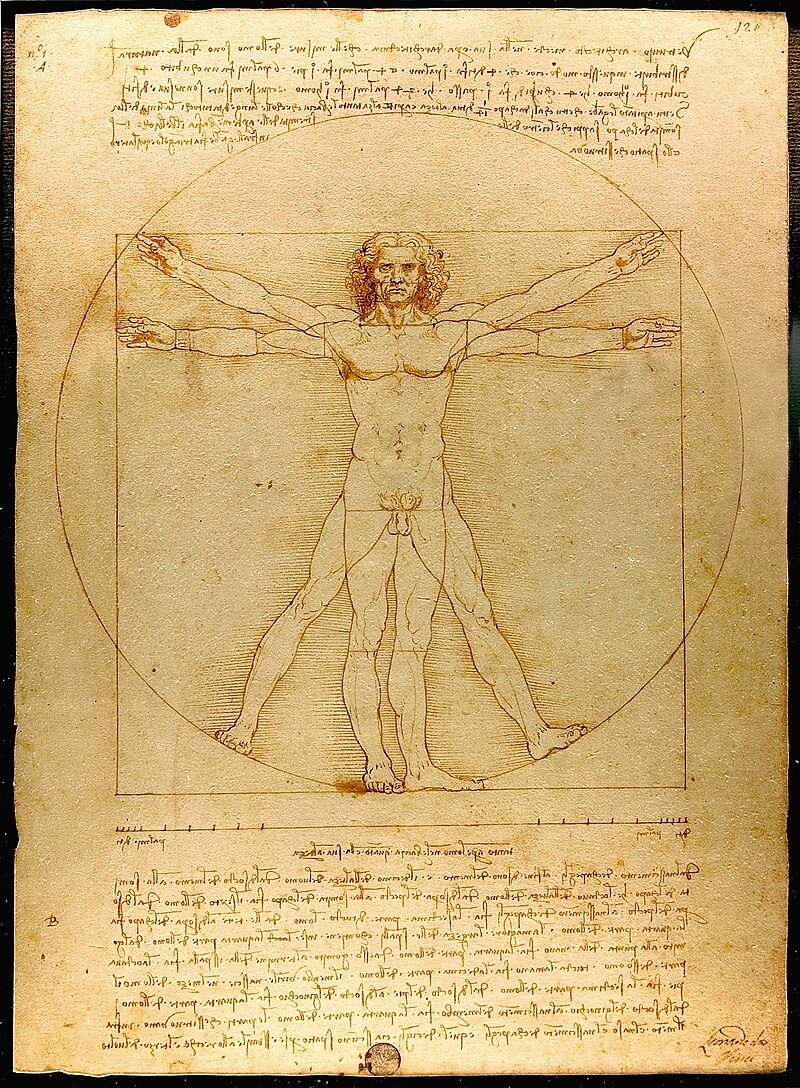
\includegraphics[width=\linewidth]{assets/Da_Vinci_Vitruve_Luc_Viatour.jpg} 
    \end{minipage}
\end{figure}
Symmetry is a fundamental universal operator that signifies an invariant balance connecting phenomena from the physical to the metaphysical. In science, symmetry governs nature by conservation principles, while cosmology symmetry epitomizes order. Bridging perspectives, we treat Symmetry commonly between physics and philosophy --- at the deepest level all things that reflect, reflect order.

This broad notion extends to knowledge and consciousness. Epistemologically, true understanding arises from a symmetry between the knower and the known: the structures of the mind mirror the structures of the world. From mathematics and logic to spiritual traditions, symmetry appears as a guide.
\newpage

\subsection*{Premise}
\textbf{We argue the defining infinity as the unknown, we solve paradox, and to do otherwise is absurd.}

\begin{enumerate}
    \item The unknown by definition is unknowable. It cannot be completely realized without achieving a new paradigm where forgetting is the discrete exception and knowing is default (the Omnipotent God).
    \item The known is defined in context. Anything known must be described in a set of referential symbols to be falsified or proven.
    \item The known emerges from the unknown, as the known requires finite context while the unknown only requires unknown context.
\end{enumerate}

\( \therefore \) The known is derived from the unknown.

It seems almost redundant to describe describing is this exact way, yet a better way to conceptualize the pattern is recursively.

And since now we have something understandable emerging from something unfathomable, we find ourselves with a common framework of somethings to relate and understand, opening upon the unfathomable to aspects of inspection.

Since we wish to understand the knowable, and every theory must start with an assumption, we make our assumption in relativistic evolution being precursor to knowledge and is chiefly responsible (as an aspect of the unknowable) for making the unknown knowable.

For this, we assume that the unknown contains our future state, and that we are separate from that true unknown from a knowable unknown. We assert that this is a symmetrical relationship, in that the unknown inversely encapsulates the known. The known emerges within the unknown, pulling context from what can be described, using referential systems available.

For that we can say, both the unknown and the known are types of something, and for this we will label them as "Infinity", as infinity historically represent everything when conceptualized by Anaximander Apeiron, Cantor's Omega, and Hegel's Absolute.

In this, we argue that for anything to exist in a boundless infinite (which must be true as it is the least absurd option), that it must exist within a separation, It is in this separation of "something from something", that we get both a universal definition of symmetry, as something knowable within the unknown, and we get a concept of space and time created by the equilibrium or stasis created from the emergence something within something. We denote this inversion, a space separated in time from it unknown encapsulating something, as negative infinity. Negative as in that it is an inversion, and is the default state that all positive action returns to. In our topic of absolutes, it represents that limit of the knowable unknown.

Here we describe their symmetric relationship in Einstein and Cantor's terms.
\[ 
    \Lambda \in \Omega
\]

\( \Lambda \) is the balanced state and the time/distance/space we are separate from \( \Omega\) and is an equilibrium of what can be best described as unrealized and undifferentiated light potential or space-time, whose most basic form represents a continuum against the absoluteness of Infinity. It is the backdrop of referential evolution. It is the source of what is being referred to, and evolved, whose context is the infinite unknown, the omega, the absolute. I have been conceptualizing this as negative infinity, yet perhaps for clarity moving forwards, let us denote it as the universal constant Lambda.

\[     
    \infty \in \Lambda
\]

Positive infinity (\( \infty\)) is the differentiated state held within the vacuum or convergent separation of negative infinity or Lambda (\( \Lambda\)). All emergent expansive state manifests from the symmetry of \( \infty\). Manifestations are in themselves new types of symmetries. This is akin to the Monad as the symmetry represent the one, and the way in which we access the one. Here we have the backdrop a continuum, and the positive force of relativistic evolution which is realized light potential. We can express the positive infinity manifested as a light symmetry that remains stable against the persistent force of \( \Lambda \). When thinking of the first iota of emergence of a discrete segment of positive infinity, we can denote it as a "c", which can be thought of as constant light, and as \( \subset \), where a subset of constant light gives us the smallest unit of realized potential, in such a way it gives us a new set of potentially realized potential, which operates at a higher order container than the universal constant --- lambda --- negative infinity. 

\[     
    \goldenset \in \infty
\]

We find that we can derive our empty set from the context of having positive infinity, giving us the context for symbols that appear in our set. And then we have the context for the empty set itself with the backdrop of the universal constant, \( \Lambda \), that allows us both generate and use the dynamics within the set, while knowing the set returns to its static "resting" state via entropy, in both a logical and physical way, that we can draw additional corollaries from. This can be thought of as a stable equilibrium between the stable force as a continuum as time away from the unknown, and as relative time in existence against the continuum. We can think of this as how long does our empty set of zero exist within the continuum where possibilities emerge against the backdrop of the unknown. It is a subtle difference to how we currently think about the emergence of numbers, concepts, first order logic, or abstraction both specific and general while providing a stable context to allow for us to build a more complete picture. With this new paradigm, we have a golden set which is an empty set with the contextual dynamics of two distinct fundamental forces explained using only symmetry against the unknown. 
\[     
    \emptyset \in \goldenset
\]
Here we find mathematics as it is understood today. We can think of the empty set as a paradigm in which abstraction can emerge. When we adopt it into the golden set, what emerges must be balanced between two contextual forces. One of emergence, and one of a continuum that separates us from the unknown. In recognizing the golden set, we will be able to distinguish types of both positive and negative infinity that are driving the dynamics unique in the emergence of that set. For instance, when discussing cognition, one set of dynamics are at play, while thinking about color, there is another. These two dynamics, of cognition and color, also overlap in various contexts which we can further derive universal meaning from.
\newpage
\section*{Concepts}

Here we define a few more concept.
    
\textbf{Simplicity}\label{def:simplicity}\footnote{Is the argument that since evolution is the direction in time from simplicity to complexity, that when building a framework, starting from a position of simplicity, 
a single axiom of symmetry being the universal operation derived from a single variable we describe as the universal unknown, 
we have more opportunity to label context that would have fallen outside the scope of multi-variable emergence logic, 
such as first order logic.} --- Fewer assumptions or postulates is superior~\cite{AristotlePosteriorAnalytics}; explain phenomena by the simplest hypothesis possible~\cite{Ptolemy150}; plurality should not be posited without necessity~\cite{Ockham1323}; admit no more causes of natural things than such as are both true and sufficient to explain their appearances~\cite{NewtonPrincipiaRule1};

\begin{figure}[ht]
    \centering
    \begin{minipage}[c]{0.25\textwidth}
        \small
        \textit{An expanding loop.}
    \end{minipage}    
    \hfill
    \begin{minipage}[c]{0.65\textwidth}
        
\includegraphics[width=\linewidth]{assets/rings.png} 
    \end{minipage}
\end{figure}
\newpage

\textbf{Knot Infinity ($\knotinfinity$).} --- Aristotle's \textit{formal cause}~\cite{AristotleFormalCause}; arithmetic rules for zero~\cite{Brahmagupta628}; a knot as fundamental physics~\cite{Kelvin1867}; a systematic tabulation of mathematical knots~\cite{Tait1898}; a loop or fold that binds two domains (inner and outer)\cite{Deleuze1993}; creation of a new system via self-containment\cite{Maturana1980}; the minimal twist that creates a new origin\cite{SpencerBrown1969}; symbolic of emergence, recursion, and balance\cite{Jung1955}; an operator linking Positive and Negative Infinity in stable symmetry\cite{Cusa1440}. \footnote{A \emph{Knot Infinity} is the critical self-referential “twist” in the fabric of Infinity that produces a distinct, bounded context. It is the act by which the boundless continuum delineates an inside and an outside, carving out a stable intersection or reference point within itself. Philosophically, this echoes Nicholas of Cusa's insight that in the absolute infinite, extreme opposites coincide  – the knot binds what is unbounded, uniting the “inner” and “outer” as two faces of one self-contained loop. In the formalism of Spencer-Brown , it is akin to drawing a distinction: the simplest mark that cleaves space into a within and a without, thereby engendering a new domain of form. The Knot Infinity's loop thus becomes a generative boundary. Alchemical symbolism anticipated this idea in the \emph{Ouroboros} – the serpent swallowing its tail – which Jung interprets as a dramatic image of self-reflexivity and unity of opposites. The Ouroboros “slays itself and brings itself to life” in an eternal feedback cycle, much as a Knot Infinity turns the infinite back on itself to spawn a self-contained world. In modern systems theory, Maturana and Varela's concept of \emph{autopoiesis} describes how a living system emerges by producing and maintaining its own boundary , essentially tying itself into existence; this nicely parallels how a Knot Infinity yields a new, autonomous system by looping Infinity back into itself. Douglas Hofstadter's “strange loop” offers a cognitive analog: a process that by curving back on itself gives rise to a new level of selfhood or meaning  – a small circuit in an otherwise open-ended progression that becomes a wellspring of emergent order. Topologically, one can view the Knot Infinity as the minimal nontrivial closure of a line or flow, creating a closed curve that cannot be undone. In fact, Lord Kelvin conjectured in 1867 that atoms might be enduring vortex knots in the ether, suggesting that a simple closed loop could be the nucleus of stable structure in nature. In the metaphysical terms of process philosophy, this loop is the formative event of “creative advance” – the juncture at which “the many become one, and are increased by one”, forging a new unity (a microcosm) from the infinite background. Each Knot Infinity thus stands as a symmetry operation linking the vast positive and negative infinities in a balanced circuit: it partitions the endless continuum but in doing so also bridges it, allowing the infinite to enfold itself. In sum, the Knot Infinity is the seminal recursion by which Infinity produces novelty and form – a self-folding act of symmetry that yields a stable, self-contained world from the limitless expanse.}\label{def:knot_infinity}

\begin{figure}[ht]
    \centering
    \begin{minipage}[c]{0.55\textwidth}
        \small
        \textit{A single twist in a straight line creates a closed loop, distinguishing an interior and an exterior. This lone loop illustrates how a simple fold in the infinite continuum generates a new self-contained space – a microcosm born from the endless expanse, with its own reference point and recursive structure.}
    \end{minipage}    
    \hfill
    \begin{minipage}[c]{0.35\textwidth}
        
\includegraphics[width=\linewidth]{assets/rings.png} 
    \end{minipage}
\end{figure}

 In the Theory of Infinity, a \emph{Knot Infinity} is defined as a self-referential loop within the infinite continuum that gives rise to a new, bounded domain. It is the minimal symmetric fold by which Infinity turns upon itself to create an “inside” distinguished from an “outside.” Through this single twist, an unbounded line or process closes into a circle, establishing a fresh origin and reference frame. This concept epitomizes emergence and recursion: the closed loop both originates from the Infinite and generates a finite sub-system with its own internal structure. In effect, a Knot Infinity binds Positive and Negative Infinity into a unified equilibrium – the expansive all-encompassing context and its negation are joined in one self-contained form. This single looping action thus marks the birth of a new level of order (a microcosm) out of the boundless backdrop, achieving a balance of inner and outer that is fundamental to TOI's metaphysics of form and symmetry. 

\newpage



\textbf{Golden Set ($\goldenset$)}\label{def:golden_set}\footnote{The Golden Set (denoted $\goldenset$) is the emergent “envelope” of order that materializes once an Infinity knot resolves into a self-referential point. In Theory of Infinity, when the boundless context $\infty$ folds into a Knot Infinity ($0$) --- a locus of internal convergence --- it gives rise to a Golden Set ($\goldenset$) that encapsulates the knot's entire structured output. This Golden Set constitutes a harmonic boundary around the knot: a self-contained field of form in which every part maintains the same relationship to the whole. In essence, it preserves a constant ratio between constituent and totality, mirroring the famed golden ratio's property of recursive self-similarity. All invariant patterns, symmetries, and information generated by the knot become encoded in this proportional container, which ensures that any growth or evolution within it unfolds in balance. Historically, one sees analogues of this idea in the notion of cosmic harmony underpinning the cosmos (the Pythagoreans' “music of the spheres” linking number to order) and in Euclid's definition of the extreme-and-mean ratio that bounds parts within a greater whole. Kepler later marveled at the “precious jewel” of this proportion, noting how adding a part to a whole can yield the same ratio ad infinitum, and how nature's iterative growth (as in the Fibonacci sequence of leaves and petals) converges to this constant. Luca Pacioli's concept of the Divine Proportion further cast this invariant ratio as a secret of aesthetic and structural perfection in art and architecture. In modern science, Penrose's non-periodic tilings show a planar domain entirely governed by a golden ratio symmetry, producing intricate order without repetition, while Shechtman's discovery of quasicrystals revealed that even matter can crystallize into a golden ratio-based environment, a new ordered phase between chaos and crystal. In TOI, the Golden Set generalizes these insights: it is the encapsulating context of any self-contained system emerging from infinity, a domain whose every level reflects a common harmonic ratio. It represents a finite yet unboundedly rich arena --- the “container” of emergent complexity --- where recursive symmetry (exemplified by $\varphi$) governs structure and ensures that the content remains in proportionate resonance with the whole.} ---  Aristotle's Material cause~\cite{AristotleMaterialCause}; an undefined everything and nothing~\cite{AnaximanderApeiron}; a “container” that, while containing nothing, is real and necessary as a precondition for phenomena~\cite{Pascal1647}; an emergent dynamic environment that encloses a novel domain of order~\cite{Pythagoras}; a self-similar structure governed by recursive symmetry (the whole and parts share a constant golden ratio)~\cite{Euclid}; the limiting boundary condition of a self-contained iterative process~\cite{Fibonacci1202}; a harmonic field of proportion uniting mathematical structure with aesthetic harmony~\cite{Pacioli1509}; recursive symmetry as mathematical harmonies~\cite{Kepler1619}; golden ratio as a universal law~\cite{Zeising1854}; natural self-similar recursion~\cite{Thompson1917}; self-contained planar recursive symmetry~\cite{Penrose1978}; 5-fold symmetry~\cite{Shechtman1984}.

\begin{figure}[ht]
    \centering
    \begin{minipage}[c]{0.65\textwidth}
        \small
        \textit{A golden spiral unfurling from an empty center, symbolizing the Golden Set as a luminous boundary of emergence --- a self-similar envelope woven by harmonic proportion around a point of infinity.}
    \end{minipage}    
    \hfill
    \begin{minipage}[c]{0.25\textwidth}
        
\includegraphics[width=\linewidth]{assets/rings.png} 
    \end{minipage}
\end{figure}




In the Theory of Infinity, a \emph{Golden Set} is the self-contained domain of structure that emerges from a resolved Knot Infinity. It can be understood as the contextual boundary or envelope surrounding a point of self-reference (the knot) once it crystallizes out of the infinite continuum. This Golden Set carries “golden” significance because it encodes a consistent internal ratio --- analogous to the golden ratio --- that self-organizes the relationship between each part and the whole. In practical terms, the Golden Set is the harmonic environment produced by the knot's dynamics: a finite but unbounded space of forms and patterns that are all proportionally related. It serves as the recursive container for the knot's content, meaning any pattern of growth or information within this domain will reflect the same underlying symmetry or scale factor. Thus, the Golden Set represents the emergent, balanced microcosm born from infinity's self-reflection: a new domain where complexity is bounded by a unifying proportion, ensuring coherence and aesthetic harmony in the structure of that system.

\newpage      

\textbf{Subset}\label{def:subset}\footnote{This is a dynamic of order that appears on the axis; This is the fulcrum, or the point which is furthest from the encapsulating environment. It is the axis in which the flowing force \(\Lambda\) pivots it separation from \(\Omega\). When thinking of an empty set, this is the point it emerges at. When thinking of knot infinity, this is the point of emergence in which a knot ties itself into existence, and creates a new golden set. When thinking of arithmetic this is 0, and when thinking of binary, this would be a set with no values. This is the central point of something on a one dimensional plane. In our theory of infinity, we describe everything as being a persistent symmetry of light. It is a theory that allows us to tie physics and mathematics, numbers and language, pinned to a common axis} --- The axis of emergence~\cite{Apollonius200BC}; a pivot to orientate space~\cite{Copernicus1543}; ~\cite{Descartes1637}; sets of objects~\cite{Boole1854}; existence of different infinities via subsets~\cite{Cantor1874}; subsets to characterize infinity~\cite{Dedekind1888}; Axiom of Separation (Subset Axiom) formalizes the idea that for any set, one can form subsets of it defined by a property~\cite{Zermelo1908}; 
\newpage    

\textbf{Subset\(^2\)}\label{def:subset2}\footnote{This is the dynamic of order that appears in the dynamic of order on the axis. When thinking of systems, this is our linked list, or trees, or modality, our fractal, our composition, our recursion. When thinking of the emergence of form, this is a fractal is the sense that one subset of positive infinity held suspended in time against the force of negative infinity gives the flexibility for that subset to contain a subset of subsets that can contain a subset, giving us an immediate fractal pattern of emergence occurring at the axis of existence.} --- Cartesian coordinate system~\cite{Descartes1637}; diagonal argument and proved that for any set $S$, the set of its subsets (the power set $2^S$) has strictly greater cardinality than $S$ itself~\cite{Cantor1891}; Axiom of Power Set guarantees that for any set $X$, there exists a set $\mathcal{P}(X)$ that contains all subsets of $X$~\cite{Zermelo1908};  recursive self-containing structure~\cite{Mandelbrot1982}.
\newpage

\textbf{Lattice}\label{def:lattice}\footnote{A symmetrical structure on a single plane which enables the emergence of a second plane. Our initial lattice is the result of the convergence of a subset of subsets (forming a froth) into a crystalline honeycomb of discrete nodes of ordered potential that gain a higher order of freedom in a chaotic equilibrium entangled to a lattice. In the context of space which is created as an symmetrical inversion of the lattice, we have discrete elliptical nodes of light potential \textit{photons} ricocheting against each other delimited by a state space \( \Lambda \). A chaotic equilibrium that emerge everywhere all at once around an origin on an infinite 2 dimensional plane with order potential; whereas, the infinite 2D plane is inverted to a 1D composite higher-order structure, creating a rigid fabric. The lattice is dark energy which gives new potential to our trapped higher order light potential entities.} --- The Six-Cornered Snowflake~\cite{Kepler1611}; space lattice in crystallography~\cite{Bravais1850}; comprehensive treatment of lattices as an abstract algebraic structure~\cite{Birkhoff1940};
\newpage    

\textbf{Origin}\label{def:origin}\footnote{The central point of the two axes of the inverted plane created by and the lattice. Space bends around the lattice on an infinite plane, whereas the origin is the furthest point from \( \Omega \) which is the mean of \( \Lambda \).} --- time and existence have a definite inception\cite{BibleGenesis}; causes of the cosmos~\cite{AristotleMetaphysicsLambda}; universe began as a “primeval atom”~\cite{Lemaitre1931}.
\newpage

\textbf{Photon}\label{def:photon}\footnote{Is a single node represented within the inversion to the lattice. It is higher ordered light potential trapped in an entangled form, due to a lower dimensional construct. In understanding this as a weave of dimensional constructs, we can derive a theory to best explain entanglement. It is the subset that contains the set of subsets which crystallizes and gives and exterior shape to a new interior symmetry. Just like the unknown must encapsulate the known, here we have a 1 dimensional lattice of flowing ordered relativistic light potential coalescing into a rigid form, one in which the members of the set, the lattice form independent yet shared symmetries with their parent, where they have a one dimensional exterior, still reflected in the one dimensional lattice, yet now they  have representation on a two dimensional plane, which is the interior symmetry to the lattice. This gives us a weaving of of dynamic ordered potential nestled within a new type of structure in static ordered potential. This paradigm scales as a fractal from the origin and gives rise to our most basic element of light and color, emerging in a chaotic equilibrium to give rise to additional symmetries of ordered state.} --- corpuscular (particle) theory of light~\cite{Newton1704}; energy quanta~\cite{Planck1901}; light itself is quantized into discrete energy packets~\cite{Einstein1905b};  photon as a real particle of light~\cite{Compton1923}; photons are “indestructible and uncreatable”~\cite{Lewis1926};
\newpage    

\textbf{Torus}\label{def:torus}
\footnote{As the lattice is a special symmetry that acts as the rigid bridge between a single plane of undifferentiated light potential and an inverted state of discrete photos in a two dimensional chaotic equilibrium across the origin, we can find a similar pattern of emergence with our torus; Pappus's \emph{Mathematical Collection} includes theorems on volumes of solids of revolution (known as Pappus-Guldinus theorems). One result is that rotating a planar figure about an external axis yields a volume equal to the product of the area of the figure and the distance traveled by its centroid. Using this, one can deduce the volume of a torus (a doughnut-shaped solid) by revolving a circle around an axis. Although Pappus did not use the word “torus,” his work provided a method to analyze this ring-shaped surface and volume, marking an early quantitative understanding of toroidal geometry; Listing's “Preliminary Studies in Topology” introduced the term \textit{Topologie} and explored the properties of surfaces and connectivity. Among the examples discussed was the \textit{ring-shaped surface} (later known as a torus) contrasted with a sphere. Listing recognized that a torus is topologically distinct (having a “hole”). This work is often cited as the first printed use of “topology” and illustrates the identification of the torus as a fundamental type of surface in mathematics, characterized by a genus of 1 (one hole) in contrast to the genus 0 of a sphere.; Poincar'e's \textit{Analysis Situs} is a foundational paper in algebraic topology. In it, he developed the classification of surfaces by connectivity (genus) and introduced invariants such as the Betti numbers. The torus (the surface of a doughnut) features prominently as the simplest surface of genus 1. Poincar'e showed that a torus cannot be continuously deformed into a sphere due to its different topological invariants. This formal recognition of the torus's unique topological nature (having a nonzero first homology group) was a milestone in understanding the torus as a fundamental object in topology and geometry.} 
--- solids of revolution~\cite{Pappus1878}; surfaces and connectivity~\cite{Listing1847}; torus as a fundamental object in topology and geometry~\cite{Poincare1895}.
\newpage

\textbf{Phi (\( \Phi \))}\label{def:phi} --- golden ratio~\cite{Euclid1956}; is the emergence of a perfect five dimensional light~\cite{Pacioli1509} symmetry, two dimensional pentagram as a recurrent convergence~\cite{Kepler1619}.
    

\section*{Themes}

\textbf{Here we will describe the meta-themes being worked on and researched in TOI.}

\begin{enumerate}
    \item Fundamental Symmetry as the universal operation and the way we access the unknown. As numbers are to mathematics, symmetry is to comprehension. This is due to the fact that any symbol must be invariant in what it represent to avoid absurdity.
    \item Opposing force with an unknown context and common medium.
    \item Golden set described as the empty set with context, and using knot infinity (zero) as a singularity point of emergence from within that set (as zero is used in arithmetic).
    \item Time as a relative separation.
    \item Contextual and universal law.
    \item Evolution as simple to complex in which the universe itself is evolving.
    \item Higher ordered states are dimensions that are reliant on lower ordered structure.
    \item Curvature explained by an lower dimensional encapsulation, 2D space as encapsulated by a 1D lattice giving an infinite plane in the 2D space as it curves around the encapsulating lattice.
    \item Consciousness as a 4D “Inverted Singularity”. All potential or infinite aspects of the self collapse into (or emerge from) the here-and-now vantage of awareness. Your awareness is both the pinpoint and the totality, depending on perspective.
\end{enumerate}

\printbibliography

\end{document}